\chapter{REQUIREMENTS ANALYSIS AND SYSTEM DESIGN}

\section{Introduction}

The Systems Development Life Cycle explicitly outlines that the Requirements Analysis Phase is the foundation upon which all successful software projects are built. As such, given both the complexity and risks present within a large event environment, this phase becomes even more critical. The failure to identify and document specific ``edge cases'' (i.e., loss of communication with a payment terminal during the middle of a transaction, or two wait staff making modifications to the same ticket) may result in potential financial discrepancies or disruptions.

Compared to corporate settings, where the collection of requirements occurs via multiple, structured interviews conducted over a long term, the event environment has a much different dynamic. The system will serve two purposes: it will act as a hard, non-elastic ledger system for the event organizer's financial needs, and it will be utilized as a soft, flexible interface for use by untrained temporary employees. This chapter will detail the conversion of problem statements into specific architectural specifications.

\section{Development Methodology}

The development of the localized OMS in environments characterized by instability or ``hostile'' network conditions requires flexible and iterative methodologies. The complexity and variability of such networks make traditional linear models, such as Waterfall, unsuitable, as they do not support rapid adjustments to the system's design or architecture. An Agile/Scrum methodology has been selected as the methodology to direct the OMS Software Development Life Cycle \cite{scrum2020guide}, an incremental approach to software development and Agile methodologies. In Agile, the iterative process breaks down the large engineering problem into smaller chunks of the total effort. At the end of each sprint (a short, time-boxed period during which specific work is completed), a predefined quantity of new functionality is implemented, tested, and prepared for release to production. This allows for incremental releases versus creating a detailed master plan upfront that may become obsolete after the first deployment. There are typically three main roles in Agile: the Product Owner (responsible for maintaining the Product Backlog and defining what the next release includes), the Scrum Master (responsible for the Scrum process and removing obstacles), and the Development Team (team members responsible for all disciplines needed to create the product). The development was performed through multiple two-week sprints. The sprint planning session occurs at the start of each sprint to define short term engineering objectives and select items from the Product Backlog to work on during the current sprint. After these objectives were identified, daily stand-up meetings occur so that members of the development team can discuss their status and issues relating to the technical aspects of the project. Two types of review sessions are held at the conclusion of each sprint: a sprint review meeting to demonstrate the results of the work completed during the previous sprint, and a sprint retrospective meeting to assess the process of completing that work. Both sessions provide an opportunity for iterative improvement of the system being built, but especially for improving the resilience of the system one component at a time. Figure~\ref{fig:agile_scrum} illustrates how the Scrum model can be properly utilized when developing software.

\begin{figure}[htbp]
    \centering
    % TODO: Create a diagram showing the Agile Scrum lifecycle (Sprint Planning -> Daily Scrum -> Sprint Review -> Retrospective)
    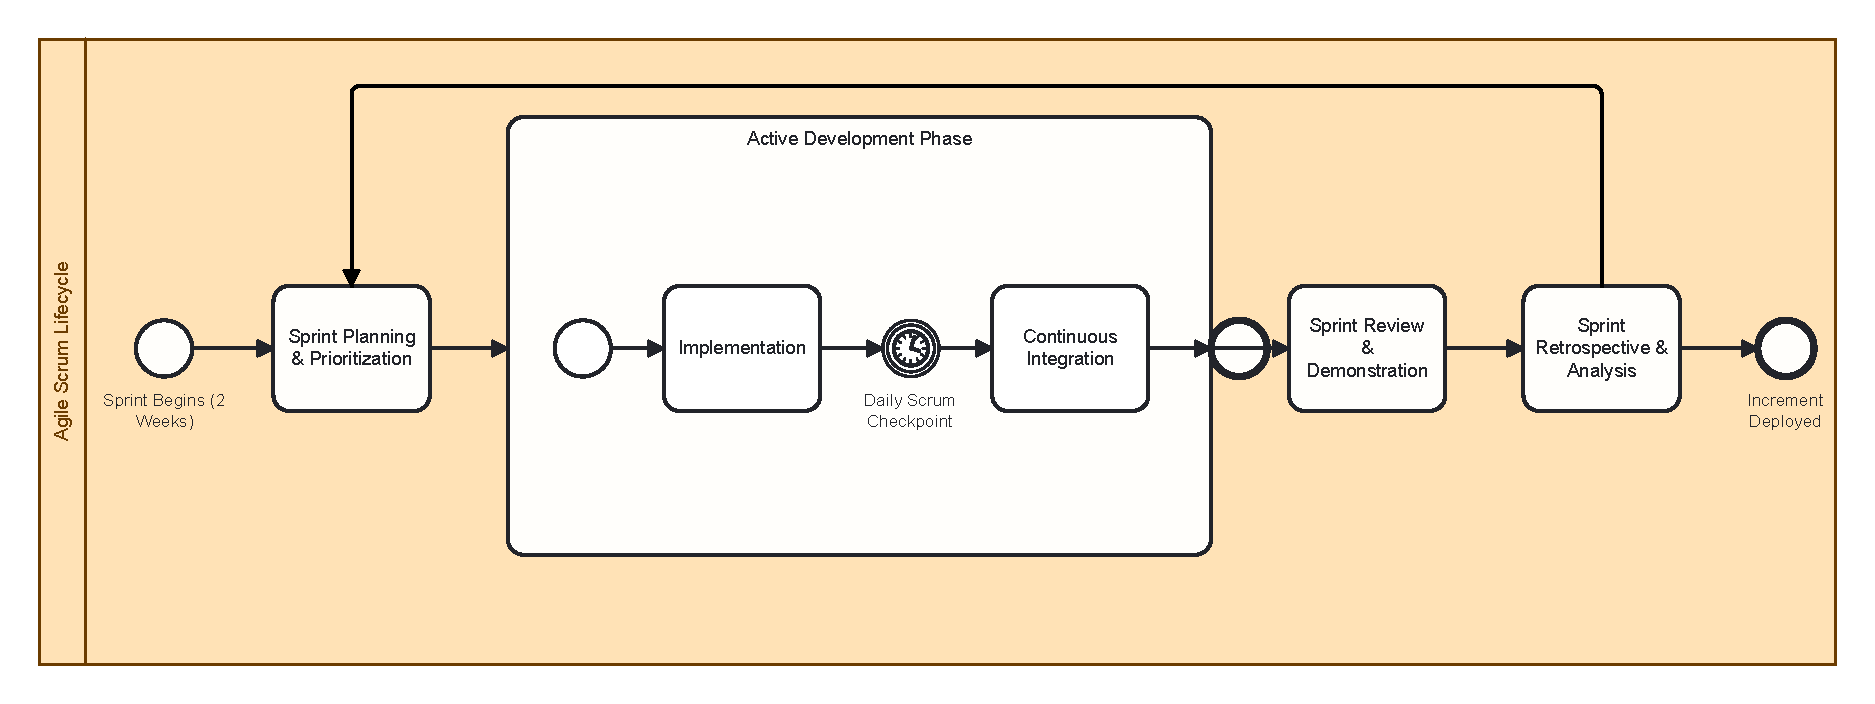
\includegraphics[width=0.8\textwidth]{images/ch3_agile_scrum.pdf}
    \caption{The iterative Agile Scrum methodology driving the continuous delivery of the developed architecture.}
    \label{fig:agile_scrum}
\end{figure}

Using this model, we had our first software development cycle to create the minimum viable core transaction loop. The first important sprint toward achieving this specific objective was to set up the base components of the hierarchical product catalog, cart logic, and RESTful order submission API. The second sprint was dedicated to building the real-time communication layer required to support both sides of the interaction. The architecture was formally documented using WebSockets instead of polling requests to enable the kitchen interface to receive updates regarding orders and to support bi-directional communication without user interaction. Finally, the last few sprints were directed toward hardening of the system and implementation of protection against edge cases that arose while running in the adversarial environment of a retail store.

\section{Stakeholder Analysis and User Personas}

In order to ensure that the deployment of the system actually fulfills all the requirements of its end-users' operational environments, we created user personas. Theoretical representations of users. These theoretical representations of users guided the design of the interfaces and the prioritization of system functions throughout the lifecycle of the project.

To guarantee that the architecture of the system will meet the performance expectations of high-volume event services, three individual user personas were created to guide the architecture. Each user persona will interact with a custom-built module within the system, designed to accommodate their own workflow and expected system behavior.

The first group, called ``cashiers,'' will sit directly in front of the line where customers physically wait. Their sole access to the system will be through an interface for entering orders and confirming payments. Because cashiers have very limited time during peak hours, the Cashier's Module has been built around maximizing speed. This has led to the use of large, high-contrast buttons (touch targets) that are organized by product category. The key expectation of this user is that there is a frictionless experience immediately when accessing the system, which will never block or freeze due to fluctuations in the network. If there is some type of transaction error condition, the system should immediately display a clearly defined degradation path from the point of error rather than a seemingly endless ``loading'' animation.

The second group includes cooks and baristas working in a production environment. While each persona interacts with the system in different ways, both are primarily information consumers who react to an incoming stream of data. The Kitchen module serves as a real-time electronic ticketing system. Cooks do not need to enter complex information, instead, they confirm whether a ticket is open and then indicate it is complete with one single tap. In order to fulfill this persona, the architecture must provide 100\% guaranteed data integrity -- a ticket can never be removed from their view until they manually complete it, and delayed tickets entered offline by cashiers must always correctly integrate into the current queue upon re-establishment of network connection.

Finally, administrators require a real-time dashboard providing a complete view of all aspects of operations. Typically located in a back-office setting, or via a mobile device while moving about, they monitor in real-time such things as current sales velocity, what products are quickly being depleted, and which cashier nodes may have issues connecting to the network. Because of this need for continuous dynamic updates to visualizations, the Administrator module heavily depends on reactive capabilities provided by an event-driven architecture in order to update visualizations dynamically without the administrator needing to continuously manually reload web pages.


\begin{figure}[htbp]
    \centering
    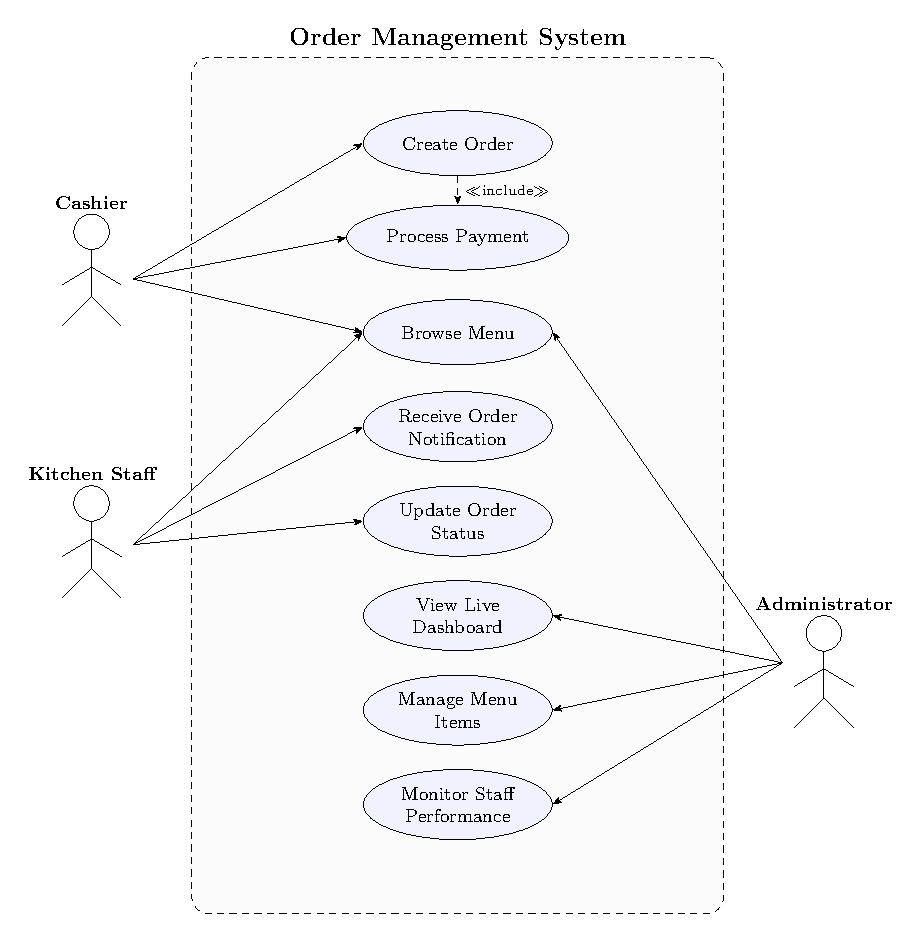
\includegraphics[width=0.85\textwidth]{images/ch3_usecase_diagram.pdf}
    \caption{UML Use Case Diagram illustrating the primary interactions between the three identified user personas and the core system functionalities.}
    \label{fig:usecase_diagram}
\end{figure}

\section{Functional Requirements}

To meet the various operational needs of the chosen environment, the system was created with a number of important functional requirements. The design of the architecture must allow for multi-channel order entry. This means the system will be able to generate and instantaneously send orders through different business areas (e.g., cash registers, kitchen, etc.). Additionally, the system will have to allow for dynamic product customization in order to accommodate multiple levels of products. This would enable a cashier to make adjustments to product ingredients or add comments on the fly when creating an order.

The first step after an order has been entered into the system, is that it will need to automatically route sub-sets of the order based on intelligent logic to direct them to the right area(s) where they can be prepared. For example, if you are preparing food at a restaurant kitchen, the items that go into preparation should only show up on your screen. There also must be some type of real-time life cycle management to track all transactions continuously and reflect all states of change from pending to handing off the last item. Lastly, one of the most important elements is high throughput, this means the capability to process an extremely large volume of orders per minute while maintaining adequate capacity and never losing or degrading the data.

\subsection{System Workflow Description}

To begin, system processes are built to model the main business functions of each persona. At a very high level, the workflow begins at checkout, where the cashier creates a new order at the point-of-sale. The cashier will then select products from the product catalog displayed at the point-of-sale. When the products have been added to the shopping cart and the total has been entered, the cashier will click ``checkout,'' proceed to payment, and the system will perform a ``handshake'' with an external payment terminal. Upon receiving a positive encrypted response from the banking gateway, the system will create a new sequential human-readable order number, record the confirmed order into an immutable MongoDB data store, and broadcast an order event via WebSockets to each of the waiting kitchen tablets so the kitchen will know to prepare the new order. Special cases are also handled. For example, if an order for the last item in stock by the cashier, prior to having time for the local terminal to confirm payment, the system will check whether stock is sufficient. If the stock is insufficient, the order will be denied, the item will not be sold, and the cashier will be asked to replace it or find another method of selling the item. These business processes were modeled using BPMN, as described above, and formally presented in Figure~\ref{fig:bpmn_order_flow}.

\begin{figure}[htbp]
    \centering
    % TODO: Ensure the BPMN diagram (from bpmn.io) for the Order Creation Flow is placed here
    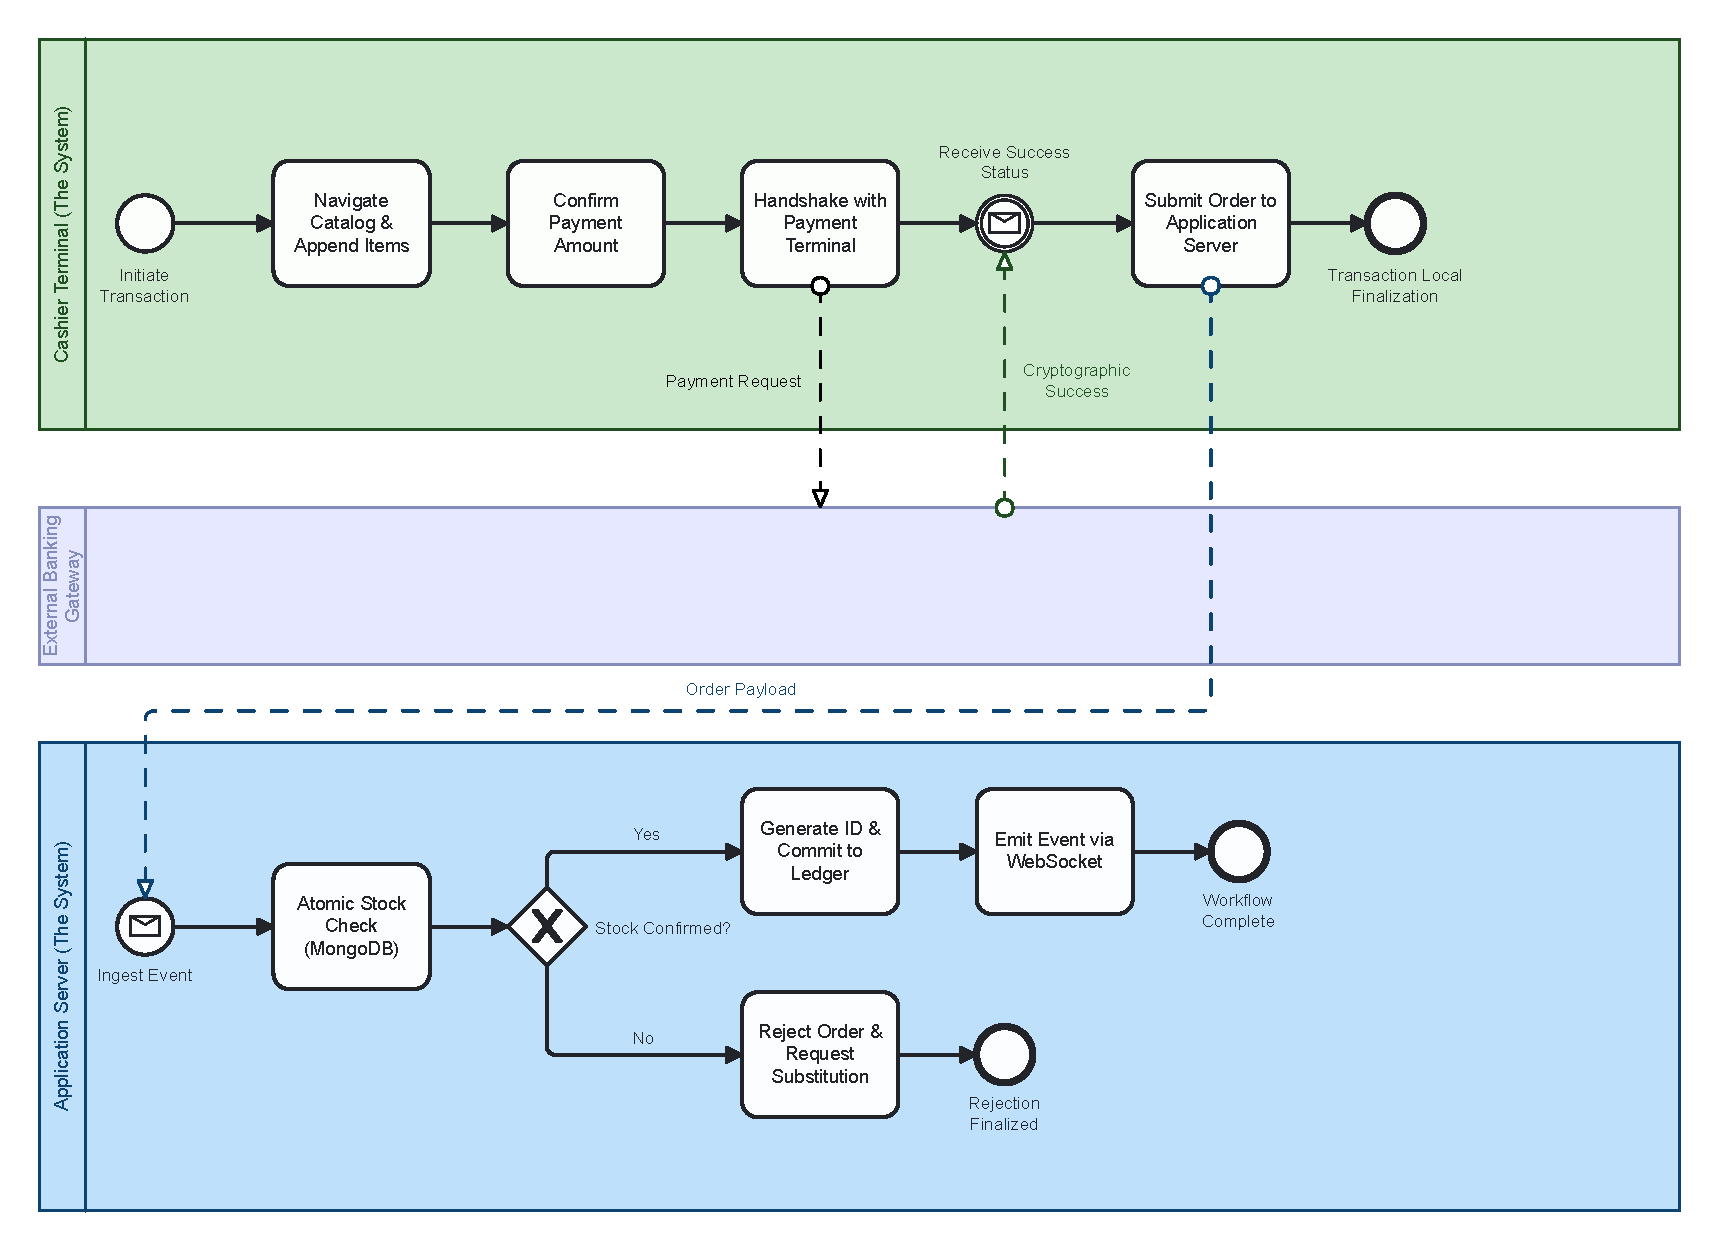
\includegraphics[width=0.9\textwidth]{images/ch3_bpmn_order.pdf}
    \caption{BPMN Model depicting the logical flow of Order Creation, from cashier input to database persistence.}
    \label{fig:bpmn_order_flow}
\end{figure}

The kitchen interface represents a separate workflow from those processed by the cashier. In the kitchen, the interface receives instantaneously a notification of each new confirmed order, displays any special preparation notes, and sounds an audible alert to notify workers when a new order is entered. Using macro-gestural inputs, the chef goes through each process state of their work from pending state to completion state. This allows us to represent the different process states of the chef in the BPMN diagrams shown in Figure~\ref{fig:bpmn_kitchen_flow}.

\begin{figure}[htbp]
    \centering
    % TODO: Ensure the BPMN diagram (from bpmn.io) for the Kitchen Display Flow is placed here
    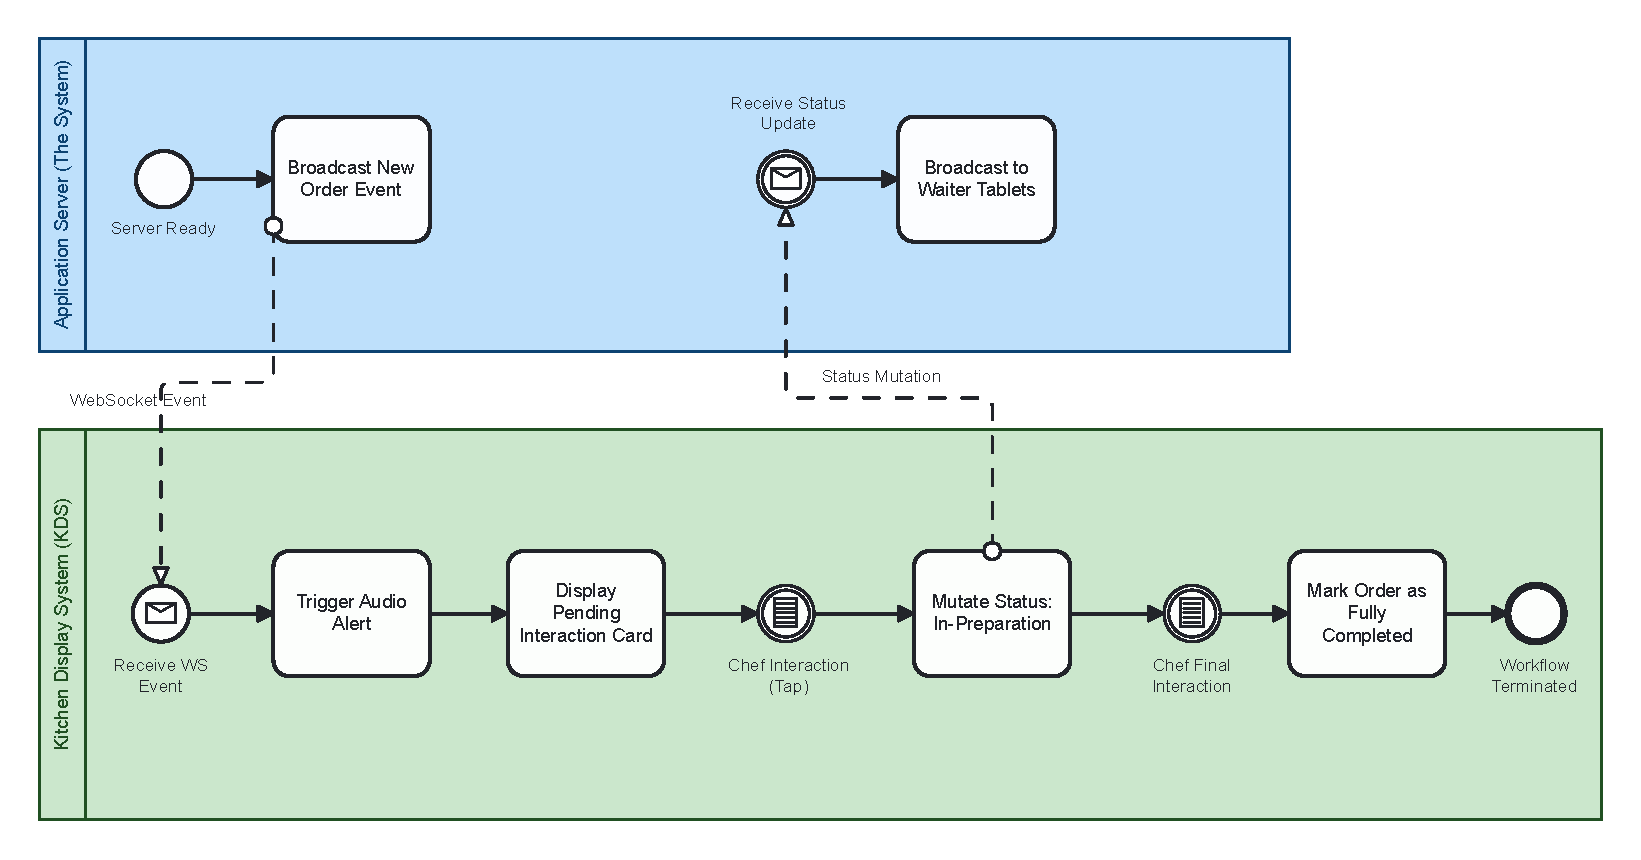
\includegraphics[width=0.8\textwidth]{images/ch3_bpmn_kitchen.pdf}
    \caption{BPMN Model depicting the Kitchen Display workflow, detailing real-time event reception and order fulfillment.}
    \label{fig:bpmn_kitchen_flow}
\end{figure}

For kitchen order management, the client application running on the kitchen tablet and the Node.js server must be in the same secure WebSocket room. When a confirmed order notification is sent from the Node.js server, the kitchen tablet receives an audible sound alert and a card for the order is added to the pending column of the user interface with corresponding animation. Once the user has selected a card to be prepared, the UI will indicate that the card is being prepared and the server will send a server push message to all waiter tablets that the card is being prepared. This completes the loop between service staff and the kitchen.

Inventory levels should be maintained based on ingredient requirements rather than goods available for final sale. For example, in regards to a burger, there are only three ingredients needed: buns, patties, cheese. Therefore, when a customer purchases a burger, you need to decrement each ingredient one at a time. The additional challenge here is if any key ingredient reaches zero, the availability of all products is immediately removed from all point-of-sale terminals. During initial play testing, it was discovered that failing to account for all components while completing a transaction would cause discrepancies in inventory count.

\section{Non-Functional Requirements}

Functional requirements explain what this System will do. Non-functional requirements represent how well this System will function when subjected to extreme operating conditions. All the restrictions are compared to current architectures \cite{iso25010}. 

Performance: The key path (the amount of time to confirm a payment and then send the confirmation message to the kitchen display) will require near-instantaneous execution without noticeable delay. Resource utilization: The Core Server Process will not consume more resources than the average commodity hardware has available (cpu, memory, disk space), and can support up to 100 concurrent clients, of which up to 50 may maintain persistent WebSocket connections simultaneously. The infrastructure must also maintain a minimum of 60 frames per second throughout the entire UI.

To force the restarting of the local servers, the reliability requirements dictate that all Active Clients will be able to connect to the local server again within 5 seconds. To avoid the ``thundering herd'' problem (all active clients connecting to the local server simultaneously) an exponential back-off algorithm is utilized. 

The system must implement database journaling and strict write concerns to ensure that financial information remains valid even if there is a loss of power immediately following an operation having been completed. Learnability is also defined as a critical non-functional requirement. For example, the system must enable a temporary employee to successfully complete a transaction independently within 5 minutes of initial use. In addition to error prevention, secondary manager authorization is also utilized for destructive operations (i.e., delete logged orders, cash refunds, etc.) to prevent accidental or malicious actions by someone utilizing the system. 

The stateless security policies that restrict a physical waiter's ability to create something via an API call (all API calls will contain a JSON Web Token and role based permissions will be applied on the first router level) will prohibit a waiter from making a request to change a product's price \cite{ferraiolo1992rbac}.

\section{Data Modeling and Schema Design}

The success of a Node.js-based API depends largely upon the efficiency of its underlying data structures. When functioning in a high volume transactional environment, an improperly structured relational query quickly becomes a system bottleneck.

For our Order Management System (OMS), we use a NoSQL approach using MongoDB \cite{banker2011mongodb} where we prioritized read/write speeds over heavy normalization. We use a somewhat denormalized document structure. In our system, for instance, we don't just insert the itemId into an order line and force the database to pull off an expensive JOIN every single request in order to get the price and name of the item - we embed the fundamental qualities of the item into the Order document at the exact time of the initial retail transaction. In doing so, we essentially lock the orders to exactly what they were at the time of purchase in the event the actual menu item is later configured to a different price. It also extensively lowers the computational cost associated with searching large order histories.

\begin{table}[htbp]
\centering
\caption{Primary Database Schema Structures for Orders and Menu Items}
\label{tab:schemas}
\begin{tabular}{@{}lll@{}}
\toprule
\textbf{Collection} & \textbf{Key Fields} & \textbf{Data Type / Relation} \\ \midrule
\texttt{Order} & \texttt{orderNumber} & String (Unique) \\
 & \texttt{status} & Enum (pending, preparing, ready, etc.) \\
 & \texttt{items} & Array of \texttt{orderItemSchema} \\
 & \texttt{totalAmount} & Number \\
 & \texttt{paymentMethod} & Enum (cash, card, iris, etc.) \\ \midrule
\texttt{MenuItem} & \texttt{name} & String \\
 & \texttt{price} & Number \\
 & \texttt{category} & ObjectId ref: \texttt{Category} \\
 & \texttt{available} & Boolean \\
 & \texttt{stock} & Number \\ \bottomrule
\end{tabular}
\end{table}

Table~\ref{tab:schemas} outlines the primary transactional schema structures utilized in the database. The complete database schema also encompasses supplementary entities, including Users (for role-based access control), Categories, and Ingredients, which are essential for full system operation.

\section{System Architecture and Component Interaction}

The architecture of our Order Management System (OMS) follows a strict decoupling between the client and server. The client, a Single Page Application (SPA), created with React, oversees all elements of the application's user interface, including user routing and the presentation of information. Our Node.js and Express RESTful API acts as our service tier, taking business logic, database queries and security, and completely separates it from the user interface.

To facilitate communication between the React frontend and the Node.js backend, a unified gateway layer built on Axios \cite{axios} was developed. To ensure security, all asynchronous requests from the client include a JSON Web Token (JWT) in the HTTP Authentication Header, which serves as a stateless handshake, cryptographically authenticating the user’s identity and specific roles without requiring the server to look up the session state in the database. Because it is completely separated from the database and session server, the backend API can be scaled independently, or replaced completely by a different language stack without requiring significant modification to the client codebase.

\section{Real-Time Communication Protocols}

The need for real-time data processing in an Order Management System (OMS) performs far better than HTTP polling, an HTTP polling use case for this example would include the client sending many requests to the server requesting new tickets to send. At high volumes, HTTP polling will have both latency and network overhead. To improve both latency and network overhead, we utilize real-time, bidirectional communication (WebSockets) by adding the Socket.io library. This establishes a bidirectional communication pipeline between all clients and servers. All non-real-time related functionality (such as static configuration data), that do not require communication via WebSockets (for example REST APIs) are utilized. Once authenticated on the socket connection, the clients subscribe to multiple ``communication rooms'' based upon their role and current service usage (for example, a cook subscribes to the `kitchen` room) \cite{socketio2024rooms}. When the API processes an order, it emits an `orderCreated` Socket.IO event into the `kitchen` Socket.IO room that the React frontend has subscribed to. The React frontend then updates its Zustand state tree in memory and triggers a full page update with the latest ticket information. This entire process takes place within milliseconds and is vastly superior to a polling-based solution.

\begin{table}[h]
\centering
\caption{WebSocket Event Specification}
\label{tab:websocket}
\begin{tabular}{|l|p{3.5cm}|p{6.5cm}|}
\hline
Event Identifier & Target Room & Operational Result \\ \hline
\texttt{new-order} & kitchen\_staff & Delivers the full order object and triggers the audio alert. \\ \hline
\texttt{order-status} & service\_staff & Updates the visual pickup board with the prepared item. \\ \hline
\texttt{scarcity-alert} & cashier\_terminals & Forces the immediate disablement of out-of-stock product buttons. \\ \hline
\end{tabular}
\end{table}

\section{Application Programming Interface (API) Specification}

A powerful RESTful API will be required to call the CRUD (Create, Read, Update, Delete) methods for system configuration and historical data as well as implement the complex first-order business logic and validation. The API adheres to the REST standards and RESTful API guidelines. All API endpoints utilize the standard HTTP verbs (GET, POST, PUT, DELETE) to communicate with logical resources. In addition to that, all API endpoints have the prefix \texttt{/api/v1/}, making it easy to perform future versions without breaking existing clients. By isolating this complex validation logic in these API controllers, we keep the database organized and uncluttered, while keeping our WebSocket layer very lightweight and only responsible for fast messaging.

\begin{table}[h]
\centering
\caption{REST API Interface Specification}
\label{tab:rest_api}
\begin{tabular}{|l|p{3cm}|p{2cm}|p{6cm}|}
\hline
Method & Endpoint & Access & Description \\ \hline
POST & /api/auth/login & Public & Authenticates user credentials and issues a secure JWT. \\ \hline
GET & /api/products & All Roles & Fetches the complete product catalog for local caching. \\ \hline
POST & /api/orders & Cashier & Creates a new order entry and fires internal socket triggers. \\ \hline
PUT & /api/orders/:id & Kitchen & Updates a specific order's status (e.g., from pending to ready). \\ \hline
GET & /api/reports & Admin & Generates comprehensive financial aggregations for dashboards. \\ \hline
\end{tabular}
\end{table}

\section{Security Architecture and Access Control}

A comprehensive approach to security is taken because of the possibility of the server being exposed to an insecure Local Area Network (LAN), thus the use of a Zero Trust Architecture Design Strategy is employed. All incoming requests to the server are viewed as potentially malicious, regardless of their origin within the LAN. When a user logs in, the server generates a JSON Web Token (JWT) that verifies user credentials \cite{ferraiolo1992rbac}. Following login, the server creates a cryptographically generated token, using the user's unique ID and role, which is then passed to the client, who stores it locally. Although the server retains no session data, any subsequent requests made to the server require a valid signature to exist on the original token. A stateless system is critical for building a fault-tolerant system. If the Node server fails and restarts while an event is occurring, it will lose ``active sessions'' since everything relies on cryptographic authentication, not on the state of the server.

Using middleware that utilizes Role-Based Access Control (RBAC), access to resources is controlled prior to the application logic processing the request (i.e., deleting a menu item). The RBAC middleware checks the JWT to see if the roles included in the JWT (i.e., admin) contain sufficient privileges to allow access to the requested resource. If it finds insufficient privilege, it returns a ``403 Forbidden'' HTTP status code and rejects the request. This prevents unauthorized modifications of stateful data at the outermost API boundary. Security logic should always be separated from application logic, never mixed together.

\begin{figure}[htbp]
    \centering
    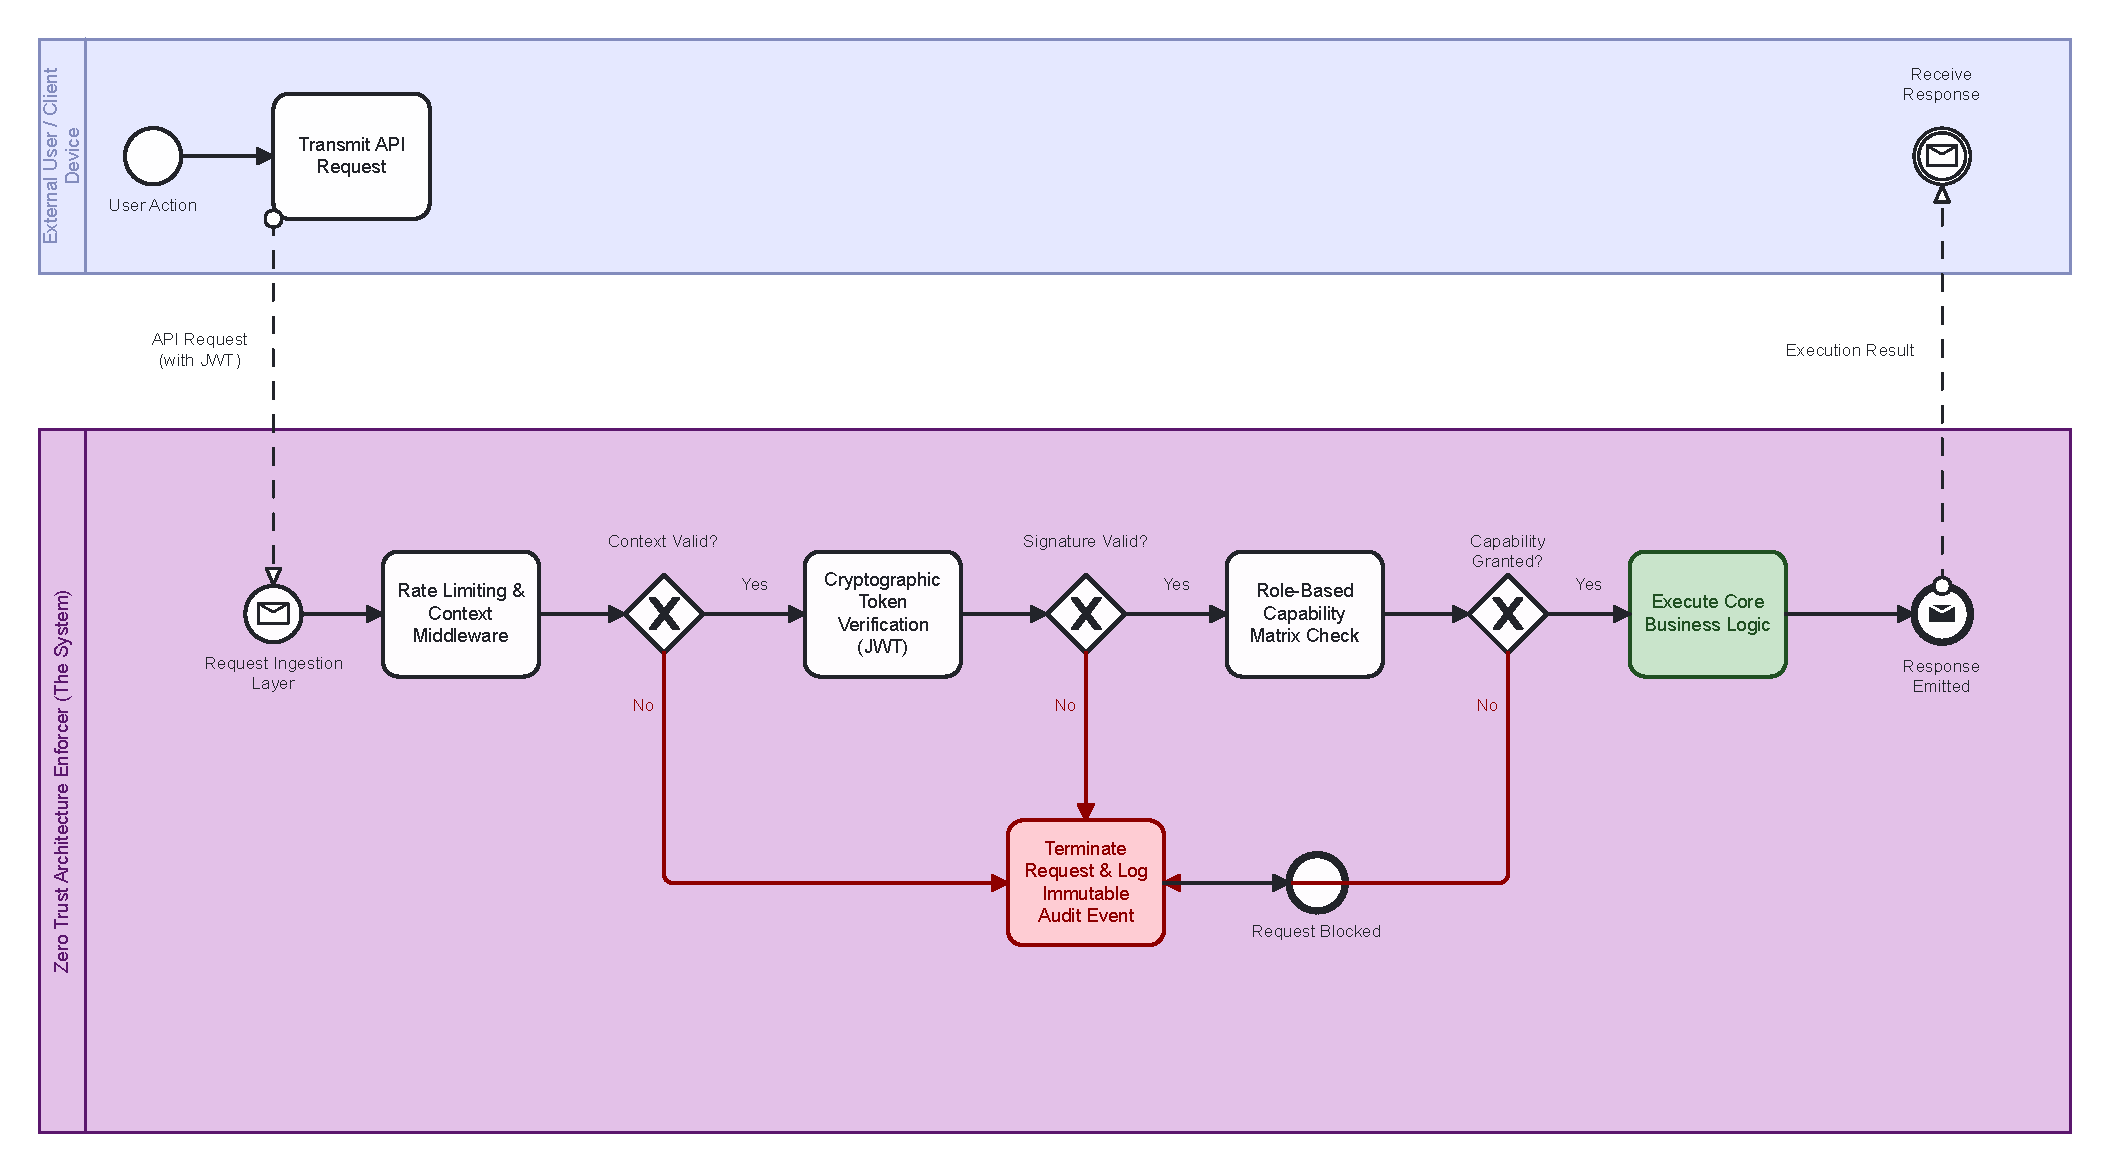
\includegraphics[width=0.9\textwidth]{images/ch3_zta_diagram.pdf}
    \caption{The Zero Trust Architecture of the system, enforcing strict capability-based authorization at every interaction layer.}
    \label{fig:zta_architecture}
\end{figure}

Additionally, a full threat modeling analysis was performed several times during the development lifecycle. Threat modeling tools from industry-standard sources were utilized to help identify and classify threats. One example of these tools is STRIDE. The word STRIDE represents Spoofing, Tampering, Repudiation, Information Disclosure, Denial of Service, and Elevation of Privilege.

Impersonation or identity theft or masquerading is referred to as spoofing. Through the utilization of cryptographically generated JSON Web Tokens (JWTs) with short expiration dates and validating signatures at each API endpoint, the risk of spoofs is greatly reduced. Because of these methods, even if an intercepted JWT is obtained in transit it is essentially worthless because it would expire almost immediately due to its expiration date.

An attacker may try to modify the product price somewhere in the checkout path, either before sending it to the customer or after receiving it from the customer while traveling to the payment gateway. The solution described here protects against this type of attack by way of an absolute validation process. Rather than relying solely on the total price value sent from the client UI to the backend API, the backend API uses a database-based pricing model as the sole trusted source.

In an extreme case, a dishonest entity could deny performing an action although there exists proof that it occurred (a cashier takes physical money from a customer but later claims ignorance regarding how an item was removed from inventory). These types of risks can be completely mitigated by establishing an immutable, append-only database that records each logical operation, including the cashier ID and timestamp of each operation.

Information disclosure occurs when any sensitive information stored in internal data (i.e., database) is returned to client systems via queries. By preventing raw MongoDB document object representations from being returned to client systems via public API calls by utilizing Data Transfer Objects (DTOs) that provide only relevant data while excluding internal fields containing sensitive information from the final JSON string transmitted over the wireless network, we prevent this problem at the database driver level.

Denial of service and elevation of privilege are handled separately. Any brute-force password guessing algorithms attempting to log into a legitimate account located onsite will be rejected by aggressive rate limiting middleware that restricts any hardware MAC address from making more than a maximum number of web requests per second. Only valid privilege boundaries are defined and enforced through middleware reviewing the context of active users. Thus, under no circumstances will a cashier-generated token ever invoke a manager-level endpoint (and vice versa).
